\documentclass[a4paper]{article}

\usepackage{bold-extra}
\usepackage[T1]{fontenc}

%\usepackage[medium]{titlesec} % Smaller section's font
%\usepackage{parskip} % To avoid indentation
\usepackage{indentfirst}
\usepackage{textcomp} % To have \textcelsius and other symbols
\usepackage[format=hang, labelformat=parens]{caption}
\usepackage{etoolbox}
\usepackage[showframe=false, top=3cm, bottom=3cm, left=3cm, right=3cm]{geometry}

\usepackage[pdftex,
pdfauthor={Davide Cossu},
pdftitle={Geometria 1},
pdfsubject={Matematica},
pdfkeywords={matematica, formulario, formule},
pdfproducer={LaTeX with hyperref},
pdfcreator={pdflatex with hyperref}]{hyperref}
\hypersetup{%
  colorlinks,
  citecolor=black,
  filecolor=black,
  linkcolor=blue,
  urlcolor=black
}
\usepackage[all]{hypcap} % To fix caption loading of hyperref

%\setcounter{secnumdepth}{0} % sections are level 1
\setcounter{tocdepth}{3}

% For better visual in tables
%\renewcommand*{\arraystretch}{2.5}

\usepackage{amsmath,amsfonts,amssymb,mathtools,mathrsfs,amsthm}
\numberwithin{equation}{section}

\usepackage{physics} %http://distrib-coffee.ipsl.jussieu.fr/pub/mirrors/ctan/macros/latex/contrib/physics/physics.pdf

\usepackage[pdftex,dvipsnames,table]{xcolor} % Colors for text
%\usepackage{xcolor}
%\usepackage{mathabx} % For better \land, \lor and \lnot
\usepackage{bm}
\usepackage{cancel}
\usepackage{siunitx}

\usepackage{tikz}
\usepackage{pgfplots}
\pgfplotsset{compat=1.14}
\usepgfplotslibrary{fillbetween}
\usepgfplotslibrary{external}
\tikzsetexternalprefix{figures/}
\tikzexternalize
\usetikzlibrary{%
  arrows,
  decorations,
  decorations.pathmorphing,
  decorations.markings,
  calc,
  intersections,
  matrix,
  spy,
  shapes.geometric,
  shapes.misc,
  patterns,
  math
}
\usepackage{tkz-euclide}
\usepackage{tikz-qtree}
\usepackage[siunitx]{circuitikz}
% http://texdoc.net/texmf-dist/doc/latex/circuitikz/circuitikzmanual.pdf
\usepackage{tikz-3dplot}

% axis style, ticks, etc
\pgfplotsset{every axis/.append style={%
    axis lines=middle,     % put the axis in the middle
    axis line style={->}, % arrows on the axis
    xlabel={$x$},          % default put x on x-axis
    ylabel={$y$},          % default put y on y-axis
    zlabel={$z$},          % default put z on z-axis
    axis equal,            % 1:1 ratio
    grid=both,             % coordinate grid
    grid style={line width=.1pt, draw=gray!10},
    major grid style={line width=.2pt,draw=gray!50},
    ticks=both,            % ticks for integers
    minor tick num=5,      % number of subticks
    ticklabel style={font=\small,fill=white},
    xlabel style={at={(ticklabel* cs:1)},anchor=north west},
    ylabel style={at={(ticklabel* cs:1)},anchor=south west},
    zlabel style={at={(ticklabel* cs:1)},anchor= west},
  }
}

\tikzset{>=stealth}
% Integral bars
\pgfplotsset{%
  integral segments/.code={\pgfmathsetmacro\integralsegments{#1}},
  integral segments=3,
  integral/.style args={#1:#2}{%
    ybar interval,
    domain=#1+((#2-#1)/\integralsegments)/2:#2+((#2-#1)/\integralsegments)/2,
    samples=\integralsegments+1,
    x filter/.code=\pgfmathparse{\pgfmathresult-((#2-#1)/\integralsegments)/2}
  }
}

\makeatletter
\def\parsenode[#1]#2\pgf@nil{%
  \tikzset{label node/.style={#1}}
  \def\nodetext{#2}
}
\tikzset{%
  % define style for the points
  Point/.style={%
    shape=circle,
    inner sep=0pt,
    minimum size=3pt,
  },
  add node at x/.style 2 args={%
    name path global=plot line,
    /pgfplots/execute at end plot visualization/.append={%
      \begingroup
        \@ifnextchar[{\parsenode}{\parsenode[]}#2\pgf@nil
        \path [name path global = position line #1-1]
        ({axis cs:#1,0}|-{rel axis cs:0,0}) --
        ({axis cs:#1,0}|-{rel axis cs:0,1});
        \path [xshift=1pt, name path global = position line #1-2]
        ({axis cs:#1,0}|-{rel axis cs:0,0}) --
        ({axis cs:#1,0}|-{rel axis cs:0,1});
        \path [
        name intersections={
          of={plot line and position line #1-1},
          name=left intersection
        },
        name intersections={
          of={plot line and position line #1-2},
          name=right intersection
        },
        label node/.append style={pos=1}
        ] (left intersection-1) -- (right intersection-1)
        node [label node]{\nodetext};
        % ---------------------------------------------------------
        % draw the tangent line from a bit right of the point on
        % the curve to the intersection with the ordinate
        % and draw the corresponding points
        %\draw [blue,thick] let
        %\p1=($ (left intersection-1) - (right intersection-1) $),
        %\p2=($ (left intersection-1)!sign(#1)*5mm!(right intersection-1) $),
        %\p3=($ ({axis cs:0,0}) - (\p2) $),
        %\n1={\p3/\p1}
        %in
        %(\p2) -- +($ {\n1}*(\x1,\y1) $)
        %%                            node [Point,fill=Tangent] (origin intersection) {}
        %%                            node [Point,fill=Curve] at (left intersection-1) {}
        %;
        %                    % ----------
        %                    % draw the horizontal line at the curve intersection point
        %                    % plus the label above/below the line
        %                    \tikzmath{
        %                        coordinate \c1;
        %                        \c1=(left intersection-1) - (right intersection-1);
        %                        \slope=\cy1/\cx1*sign(#1);
        %                    }
        %                    \pgfmathsetmacro{\AboveBelow}{ \slope>0 ? "above" : "below" }
        %                    \draw [dotted]
        %                        ([xshift=sign(#1)*2.5mm] left intersection-1) --
        %                        (left intersection-1) --
        %                            node [\AboveBelow,node font=\scriptsize] {$f(x)$}
        %                        (left intersection-1 -| origin intersection) --
        %                        +($ sign(#1)*(-2.5mm,0) $)
        %                            coordinate [pos=0.5] (a)
        %                    ;
        %                    % draw the horizontal line at the ordinate intersection point
        %                    \draw [dotted] (origin intersection)
        %                        +($ sign(#1)*(-2.5mm,0) $) --
        %                        (origin intersection);
        %                    % draw vertical line left/right of the ordinate
        %                    \pgfmathsetmacro{\LeftRight}{ #1<0 ? "right" : "left" }
        %                    \draw [stealth-stealth] (origin intersection)
        %                        +($ sign(#1)*(-1.25mm,0) $) -- (a)
        %                            node [midway,\LeftRight,node font=\scriptsize] {$p$}
        %                    ;
        %                    % ---------------------------------------------------------
      \endgroup
    },
  },
}
\makeatother

\makeatletter
\def\mathcolor#1#{\@mathcolor{#1}}
\def\@mathcolor#1#2#3{%
  \protect\leavevmode
  \begingroup
  \color#1{#2}#3%
  \endgroup
}
\makeatother
\newcommand{\Setsuchthat}{\;\ifnum\currentgrouptype=16 \middle\fi|\;}
\newcommand{\suchthat}{\,:}

% For an older but clearer root. Still \oldsqrt is valid
\usepackage{letltxmacro}
\makeatletter
\let\oldr@@t\r@@t
\def\r@@t#1#2{%
  \setbox0=\hbox{$\oldr@@t#1{#2\,}$}\dimen0=\ht0
  \advance\dimen0-0.2\ht0
  \setbox2=\hbox{\vrule height\ht0 depth -\dimen0}%
{\box0\lower0.4pt\box2}}
\LetLtxMacro{\oldsqrt}{\sqrt}
\renewcommand*{\sqrt}[2][\ ]{\oldsqrt[#1]{#2} }
\makeatother

\newcommand\markangle[7][red]{% [color] origin A B radius radiusmark mark
  % fill red circle
  \begin{scope}
    \path[clip] (#2) -- (#3) -- (#4);
    \fill[color=#1,fill opacity=0.5,draw=#1,name path=circle]
    (#2) circle (#5);
  \end{scope}
  % middle calculation
  \path[name path=line one] (#2) -- (#3);
  \path[name path=line two] (#2) -- (#4);
  \path[%
  name intersections={of=line one and circle, by={inter one}},
  name intersections={of=line two and circle, by={inter two}}
  ] (inter one) -- (inter two) coordinate[pos=.5] (middle);
  % put mark
  \node at ($(#2)!#6!(middle)$) {#7};
}

\newcommand\domainplot[3]{ % start end list \domainplot{0}{2}{0,1}
  \draw[shorten <= -1cm,shorten >= -1cm] (#1) -- (#2);
  \foreach \x in #3{
    \coordinate (A) at (#1);
    \coordinate (B) at (\x,0);
    \filldraw[fill=white,draw=black] (A-|B) circle(2pt)
    node[below]{\x};
  }
}

\newcommand{\mysign}[1]{%
  \pgfmathtruncatemacro\tmpsign{sign(#1)}
  \ifnum\tmpsign<0
  -
  \else
  \ifnum\tmpsign>0
  +
  \else
  \relax
  \fi
  \fi
}

\newcommand{\mytick}[1]{%
  \pgfmathtruncatemacro\tmpsign{sign(#1)}
  \ifnum\tmpsign<0
  \relax
  \else
  \ifnum\tmpsign>0
  \relax
  \else
  $|$
  \fi
  \fi
}

\newcommand{\drawSign}[6][]{% f(x) xmin xmax delta exclpoints
  \begin{scope}[#1,declare function={Test(\x) = #2;}]
    \draw [->, thick] (#3,0) -- (#4,0)node[right] {$x$};
    \pgfmathsetmacro{\NextI}{#3+#5}
    \foreach \i in {#3,\NextI,...,#4}{%
      \node at (\i,{0.35*sign(max(min(Test(\i),1),-1))}) {$\mysign{Test(\i)}$};
      \pgfmathtruncatemacro\signum{sign(Test(\i))}
      \ifnum\signum=0
      \filldraw[black] (\i,0) circle(2pt);
      %\node[circle,fill,maximum size=2pt] at (\i,0){};
      \node[below] at (\i,-0.2){$\i$};
      \fi
    }
    \ifx&#6&%
    \else  
    % Excluded points
    \foreach \x in #6{%
      \filldraw[fill=white,draw=black] (\x,0) circle(2pt);
      \node[below] at (\x,-0.2) {$\x$};
    }
    \fi
  \end{scope}
}

\DeclareMathOperator{\im}{im}
\DeclareMathOperator{\id}{id}

% Arc over text
\usepackage{graphicx}
\makeatletter
\DeclareFontFamily{U}{tipa}{}
\DeclareFontShape{U}{tipa}{m}{n}{<->tipa10}{}
\newcommand{\arc@char}{{\usefont{U}{tipa}{m}{n}\symbol{62}}}%

\newcommand{\arc}[1]{\mathpalette\arc@arc{#1}}

\newcommand{\arc@arc}[2]{%
  \sbox0{$\m@th#1#2$}%
  \vbox{%
    \hbox{\resizebox{\wd0}{\height}{\arc@char}}
    \nointerlineskip
    \box0
  }%
}
\makeatother

% Matrix spacing
%\makeatletter
%\renewcommand*\env@matrix[1][\arraystretch]{%
%  \edef\arraystretch{#1}%
%  \hskip -\arraycolsep
%  \let\@ifnextchar\new@ifnextchar
%\array{*\c@MaxMatrixCols c}}
%\makeatother

\makeatletter
\renewcommand*\env@matrix[1][*\c@MaxMatrixCols c]{%
  \hskip -\arraycolsep
  \let\@ifnextchar\new@ifnextchar
  \array{#1}}
\makeatother

\everymath{\displaystyle}
\newcommand\ddfrac[2]{\frac{\displaystyle #1}{\displaystyle #2}}

% Proof changes
\renewcommand\qedsymbol{QED}

\expandafter\let\expandafter\oldproof\csname\string\proof\endcsname
\let\oldendproof\endproof
\renewenvironment{proof}[1][\proofname]{%
  \oldproof[\bfseries \scshape #1]\mbox{}\\*%
}{\oldendproof}

% Hôpital's equivalence
\newcommand{\Heq}[1]{\overset{\left[#1\right]}{\underset{\mathrm{H}}{=}}}
\newcommand{\bydef}{\overset{\text{def}}{=}}

\let\oldemptyset\emptyset
\let\emptyset\varnothing

\newcommand{\notimplies}{%
\mathrel{{\ooalign{\hidewidth$\not\phantom{=}$\hidewidth\cr$\implies$}}}}

\newcommand*{\transp}[2][-3mu]{\ensuremath{\mskip1mu\prescript{\smash{\mathrm t\mkern#1}
}{}{\mathstrut#2}}}%

\usepackage[italian]{babel} % Italian support
\usepackage[utf8]{inputenc} % Accented letters
\usepackage{xtab, booktabs, array} % For better tables
\usepackage{multirow} % For nicer tables with split rows/columns
\usepackage{multicol}
\usepackage{enumitem} % For more flexibility on lists
\usepackage{xargs,xparse}
\usepackage[colorinlistoftodos,prependcaption,textsize=tiny]{todonotes}

% Some useful TODO commands
\newcommandx{\unsure}[2][1=]{\todo[linecolor=red,backgroundcolor=red!25,bordercolor=red,#1]{#2}}
\newcommandx{\change}[2][1=]{\todo[linecolor=blue,backgroundcolor=blue!25,bordercolor=blue,#1]{#2}}
\newcommandx{\info}[2][1=]{\todo[linecolor=OliveGreen,backgroundcolor=OliveGreen!25,
bordercolor=OliveGreen,#1]{#2}}
\newcommandx{\improvement}[2][1=]{\todo[linecolor=Plum,backgroundcolor=Plum!25,
bordercolor=Plum,#1]{#2}}
\newcommandx{\thiswillnotshow}[2][1=]{\todo[disable,#1]{#2}}

%\setlength{\marginparwidth}{2cm} % For better TODO's display

% To center with m{}
\newcolumntype{M}[1]{>{\centering\arraybackslash}m{#1}}


%!TEX ROOT=geometria1.tex
\newtheoremstyle{teorema}{1.5em}{1.5em}{}{}{\bfseries}{.}{.5em}{Teorema \thmnumber{#2}:
#1}
\theoremstyle{teorema}

\newtheorem{innerThm}{\envargumenta}[section]
\newtheorem{innerSubThm}{\envargumenta}[innerThm]

%!TEX ROOT=geometria1.tex
\newtheoremstyle{definizione}{1.5em}{1.5em}{}{}{\bfseries}{.}{.5em}{Definizione
\thmnumber{#2}: #1}
\theoremstyle{definizione}

\newtheorem{innerDef}{\envargument}[section]
\newtheorem{innerSubDef}{\envargument}[innerDef]

%!TEX ROOT=geometria1.tex
\newtheoremstyle{esempio}{1.5em}{1.5em}{}{}{\bfseries}{.}{.5em}{Esempio \thmnumber{#2}:
#1}
\theoremstyle{esempio}

\newtheorem{innerEx}{\envargumentb}[section]
\newtheorem{innerSubEx}{\envargumentb}[innerThm]


\newcommand{\innerDefautorefname}{Definizione}
\newcommand{\innerThmautorefname}{Teorema}
\newcommand{\innerExautorefname}{Esempio}
\newcommand{\innerSubDefautorefname}{Definizione}
\newcommand{\innerSubThmautorefname}{Teorema}
\newcommand{\innerSubExautorefname}{Esempio}

\newcommand{\envargument}{}
\newenvironment{Def}[1]
 {\renewcommand{\envargument}{#1}\innerDef}
 {\endinnerDef}
\newenvironment{SubDef}[1]
 {\renewcommand{\envargument}{#1}\innerSubDef}
 {\endinnerSubDef}

\newcommand{\envargumenta}{}
\newenvironment{Thm}[1]
 {\renewcommand{\envargumenta}{#1}\innerThm}
 {\endinnerThm}
\newenvironment{SubThm}[1]
 {\renewcommand{\envargumenta}{#1}\innerSubThm}
 {\endinnerSubThm}

\newcommand{\envargumentb}{}
\newenvironment{Ex}[1]
 {\renewcommand{\envargumentb}{#1}\innerEx}
 {\endinnerEx}
\newenvironment{SubEx}[1]
 {\renewcommand{\envargumentb}{#1}\innerSubEx}
 {\endinnerSubEx}

\begin{document}

\title{Geometria 1: appunti}
\author{Davide Cossu}
\date{2018}
\maketitle

\begin{abstract}
  Una dispensa contenente gli appunti delle lezioni di Geometria 1, con anche esempi e
  dimostrazioni.
\end{abstract}

{%
  \newpage
  \hypersetup{linkcolor=black}
  \tableofcontents
  \newpage
}

%!TEX ROOT=geometria1.tex

\section{Matrici}%
\label{sec:matrici}

\subsection{Definizioni}%
\label{sub:definizioni_e_teoremi}

\begin{Def}{Matrice}
  Siano $m,n\in\mathbb{N}_0$. Una matrice di $m$ righe e $n$ colonne ad elementi reali è
  una tabella del tipo
  \begin{equation*}
    A =
    \begin{pmatrix}[1]
      a_{1,1} & a_{1,2} & \cdots & a_{1,n} \\
      a_{2,1} & a_{2,2} & \cdots & _{2,n} \\
      \vdots  & \vdots  & \ddots & \vdots  \\
      a_{m,1} & a_{m,2} & \cdots & a_{m,n}
    \end{pmatrix}
  \end{equation*}
  con $a_{ij}\in\mathbb{R}$ e $1\leq i\leq m$ e $1\leq j\leq n$.
\end{Def}

\begin{Def}{Ordine}
  Si dice \textbf{ordine} di una matrice si intendono le sue dimensioni, in questo caso
  $A$ è di ordine $m\times n$.
\end{Def}

Dato che una matrice contiene elementi reali, l'insieme di queste matrici viene definito
\begin{equation*}
  \mathbb{R}^{m,n}\bydef \{\text{Matrici reali di ordine }m\times n\}
\end{equation*}
Spesso una matrice viene definita anche in maniera più stringata
\begin{equation*}
  A = (a_{ij})\in\mathbb{R}^{m,n}
\end{equation*}

\begin{Def}{Matrice quadrata}
  Una matrice si dice quadrata quando $m=n$.
\end{Def}

\begin{Def}{Matrice identità}
  La matrice identità (o matrice unità) si definisce
  \begin{equation*}
    I\in\mathbb{R}^{m,n}\bydef
    \begin{pmatrix}
      1 & 0 & \cdots & 0\\
      0 & 1 & 0 & \vdots\\
      \vdots & 0 & 1 & 0\\
      0 & \cdots & 0 & 1
    \end{pmatrix}
  \end{equation*}
  Ovvero quella matrice la cui diagonale principale è formata da $1$ e tutto il resto da
  $0$. Formalmente
  \begin{equation*}
    a_{ij} =
    \begin{cases}
      0, &\text{ se }i\neq j\\
      1, &\text{ se }i=j
    \end{cases}
  \end{equation*}
\end{Def}

\begin{Def}{Diagonale principale}
  La diagonale principale di una matrice è quella descritta dagli elementi $a_{ii}$. Qui
  è colorata in blu.
  \begin{center}
    \begin{tikzpicture}[baseline=(A.center), scale=0.5]
      \tikzset{node style ge/.style={circle}}
      \tikzset{bar/.style = {opacity=.3,line width=4 mm,line cap=round,color=#1}}
      \tikzset{plus/.style = {above left,,opacity=1,circle,fill=#1!50}}
      \tikzset{minus/.style = {below left,,opacity=1,circle,fill=#1!50}}

      \matrix (A) [matrix of math nodes, nodes = {node style ge}, left delimiter = (,
      right delimiter = ),column sep=0 mm]
      {a_{11} & a_{12} & a_{13}\\
        a_{21} & a_{22} & a_{23}\\
        a_{31} & a_{32} & a_{33}\\
      };

      \draw [bar=blue] (A-1-1.north west) to (A-3-3.south east);
    \end{tikzpicture}
  \end{center}
\end{Def}

\begin{Def}{Matrice nulla}
  Per matrice nulla si intende
  \begin{equation*}
    O\in\mathbb{R}^{m,n}\bydef
    \begin{pmatrix}[1]
      0&\cdots&0\\
      \vdots & \ddots & \vdots\\
      0 & \cdots & 0
    \end{pmatrix}
  \end{equation*}
  Ovvero è la matrice tale che
  \begin{equation*}
    \forall i,j \quad a_{ij}=0
  \end{equation*}
\end{Def}

\begin{Def}{Matrice riga}
  Per matrice riga si intende quella che ha $m=1$, ovvero
  \begin{equation*}
    A =
    \begin{pmatrix}
      a_{11} & \cdots & a_{1n}
    \end{pmatrix}
    \in\mathbb{R}^{1,n}
  \end{equation*}
\end{Def}

\begin{Def}{Matrice colonna}
  Per matrice colonna si intende quella che ha $n=1$, ovvero
  \begin{equation*}
    A =
    \begin{pmatrix}
      a_{11}\\
      \vdots\\
      a_{m1}
    \end{pmatrix}
    \in\mathbb{R}^{m,1}
  \end{equation*}
\end{Def}

\begin{Def}{Matrice simmetrica}
  Sia $A\in\mathbb{R}^{n,n}$. $A$ è simmetrica se $\transp A = A$. Ovvero se
  \begin{equation*}
    a_{ij} = a_{ji}\quad\forall i,j=1,\ldots,n
  \end{equation*}
\end{Def}

\begin{Def}{Matrice antisimmetrica}
  Sia $A\in\mathbb{R}^{n,n}$. $A$ è antisimmetrica se $\transp A = -A$. Ovvero se
  \begin{equation*}
    a_{ij} = -a_{ji}\quad \forall i,j=1,\ldots,n
  \end{equation*}
\end{Def}

\begin{Def}{Matrice invertibile}\label{def:matrice_inversa}
  Sia $A$ una matrice quadrata. $A$ è in vertibile o non singolare se
  \begin{equation*}
    \exists X\in\mathbb{R}^{n,n}\suchthat AX = XA = I
  \end{equation*}
  Si noti che si indica $X = A^{-1}$.
\end{Def}

\begin{Thm}{Unicità dell'inversa}
  Se $A\in\mathbb{R}^{n,n}$ è invertibile allora la matrice inversa è unica.
\end{Thm}

\begin{proof}
  Sopponiamo per assurdo che $\exists X,X'\in\mathbb{R}^{n,n}$ con $X\neq X'$ tali che
  \begin{equation*}
    AX'=X'A=AX=XA=I
  \end{equation*}
  Allora
  \begin{equation*}
    X'=IX' = (XA)X' = X(AX') = XI = X
  \end{equation*}
\end{proof}

\begin{SubDef}{Proprietà della matrice inversa}
  La matrice inversa gode di alcune proprietà:
  \begin{enumerate}
    \item $(AB)^{-1} = B^{-1}A^{-1}\quad\forall A,B\in\mathbb{R}^{n,n}$
      \begin{proof}
        Dobbiamo dimostrare $B^{-1}A^{-1}={(AB)}^{-1}\iff
          AB(A^{-1}B^{-1})=(A^{-1}B^{-1})AB=I$ per la~\autoref{def:matrice_inversa}.
          Quindi
          \begin{equation*}
            B^{-1}A^{-1}(AB) = B^{-1}(A^{-1}A)B = B^{-1}B = I
          \end{equation*}
          e
          \begin{equation*}
            AB(A^{-1}B^{-1}) = A(BB^{-1})A^{-1} = AA^{-1} = I
          \end{equation*}
      \end{proof}
    \item ${(A^{-1})}^{-1}\quad\forall A\in\mathbb{R}^{n,n}$
      \begin{proof}
        Per~\autoref{def:matrice_inversa}
        \begin{equation*}
          A^{-1}A = AA^{-1} = I
        \end{equation*}
      \end{proof}
  \end{enumerate}
\end{SubDef}

\begin{SubDef}{Gruppo lineare}
  Si definisce un gruppo lineare l'insieme
  \begin{equation*}
    GL(n,\mathbb{R})\bydef \left\{ A\in\mathbb{R}^{n,n}\Setsuchthat A\text{ è
    invertibile} \right\}
  \end{equation*}
  assieme al prodotto.
\end{SubDef}

\begin{Def}{Matrice diagonale}
  Sia $A\in\mathbb{R}^{n,n} = (a_{ij})$. Si dice diagonale se
  \begin{equation*}
    \forall i,j = 1,\ldots,n\suchthat i\neq j\quad a_{ij} = 0
  \end{equation*}
  Ovvero
  \begin{equation*}
    \mqty(\dmat[0]{a_{11}, a_{22}, \ddots, a_{nn}})
  \end{equation*}
\end{Def}

\subsection{Operazioni}%
\label{sub:operazioni}

\begin{Def}{Uguaglianza}
  Due matrici $A=(a_{ij})\in\mathbb{R}^{m,n}$ e $B=(b_{ij})\in\mathbb{R}^{p,q}$ si dicono
  uguali se
  \begin{enumerate}
    \item $A$ e $B$ appartengono allo stesso insieme $\mathbb{R}^{m,n}$, ovvero $m=p$ e
      $n=q$
    \item $a_{ij} = b_{ij},\quad\forall i:\,1\leq i\leq m \quad\forall j:\,1\leq j\leq n$
  \end{enumerate}
\end{Def}

\begin{Def}{Somma}
  La somma tra matrici è solo definita se le due matrici appartengono allo stesso
  insieme.\\
  Siano $A=(a_{ij})\in\mathbb{R}^{m,n}$ e $B=(b_{ij})\in\mathbb{R}^{m,n}$ due matrici.
  La loro somma $A+B$ è
  \begin{equation*}
    A+B\bydef (a_{ij}+b_{ij})
  \end{equation*}
  Si definisce quindi anche l'operatore somma nel seguente modo
  \begin{align*}
    +:&\;\mathbb{R}^{m,n}\times\mathbb{R}^{m,n}\rightarrow\mathbb{R}^{m,n}\\
      & (A,B)\mapsto A+B
  \end{align*}
\end{Def}

\begin{SubDef}{Proprietà della somma tra matrici}
  Per la somma tra matrici valgono le seguenti proprietà:
  \begin{enumerate}
    \item Commutativa: $A+B = B+A\quad\forall A,B\in\mathbb{R}^{m,n}$
    \item Associativa: $A+(B+C) = (A+B)+C\quad\forall A,B,C\in\mathbb{R}^{m,n}$
    \item Esistenza dell'elemento neutro: $O+A = A+O\quad\forall A\in\mathbb{R}^{m,n}$
    \item Esistenza dell'opposto: $A+(-A) = 0\quad\forall A\in\mathbb{R}^{m,n}$
  \end{enumerate}
\end{SubDef}

\begin{Def}{Prodotto tra matrice e scalare}
  Si definisce il prodotto tra $\lambda\in\mathbb{R}$ e $A=(a_{ij})\in\mathbb{R}^{m,n}$
  la matrice
  \begin{equation*}
    \lambda A\bydef(\lambda a_{ij})
  \end{equation*}
\end{Def}

\begin{SubDef}{Proprietà del prodotto con uno scalare}
  Per il prodotto tra una matrice e uno scalare vigono le seguenti proprietà:
  \begin{enumerate}
    \item $\lambda(A+B) = \lambda A + \lambda B\quad\forall\lambda\in\mathbb{R},\;
      \forall A,B\in\mathbb{R}^{m,n}$
    \item $(\lambda+\mu)A = \lambda A + \mu A\quad\forall\lambda,\mu\in\mathbb{R},\;
      \forall A\in\mathbb{R}^{m,n}$
    \item $(\lambda\mu)A = \lambda(\mu A)\quad\forall\lambda,\mu\in\mathbb{R},\;
      \forall A\in\mathbb{R}^{m,n}$
    \item $1A = A\quad\forall A\in\mathbb{R}^{m,n}$
  \end{enumerate}
\end{SubDef}

\begin{Def}{Prodotto tra matrici}\label{def:matrice_prodotto}
  Il prodotto tra due matrici $A\in\mathbb{R}^{m,n}$ e $B\in\mathbb{R}^{p,q}$ è
  possibile solo se $n=p$. La matrice risultante avrà ordine $m\times q$.
  Formalmente si scrive che
  \begin{equation*}
    C \bydef A\cdot B = (c_{ij})\in\mathbb{R}^{m,q}
  \end{equation*}
  con
  \begin{equation*}
    c_{ij} = \sum^{n}_{k=1} a_{ik}b_{kj}
  \end{equation*}
  \begin{figure}[!htbp]
    \centering
    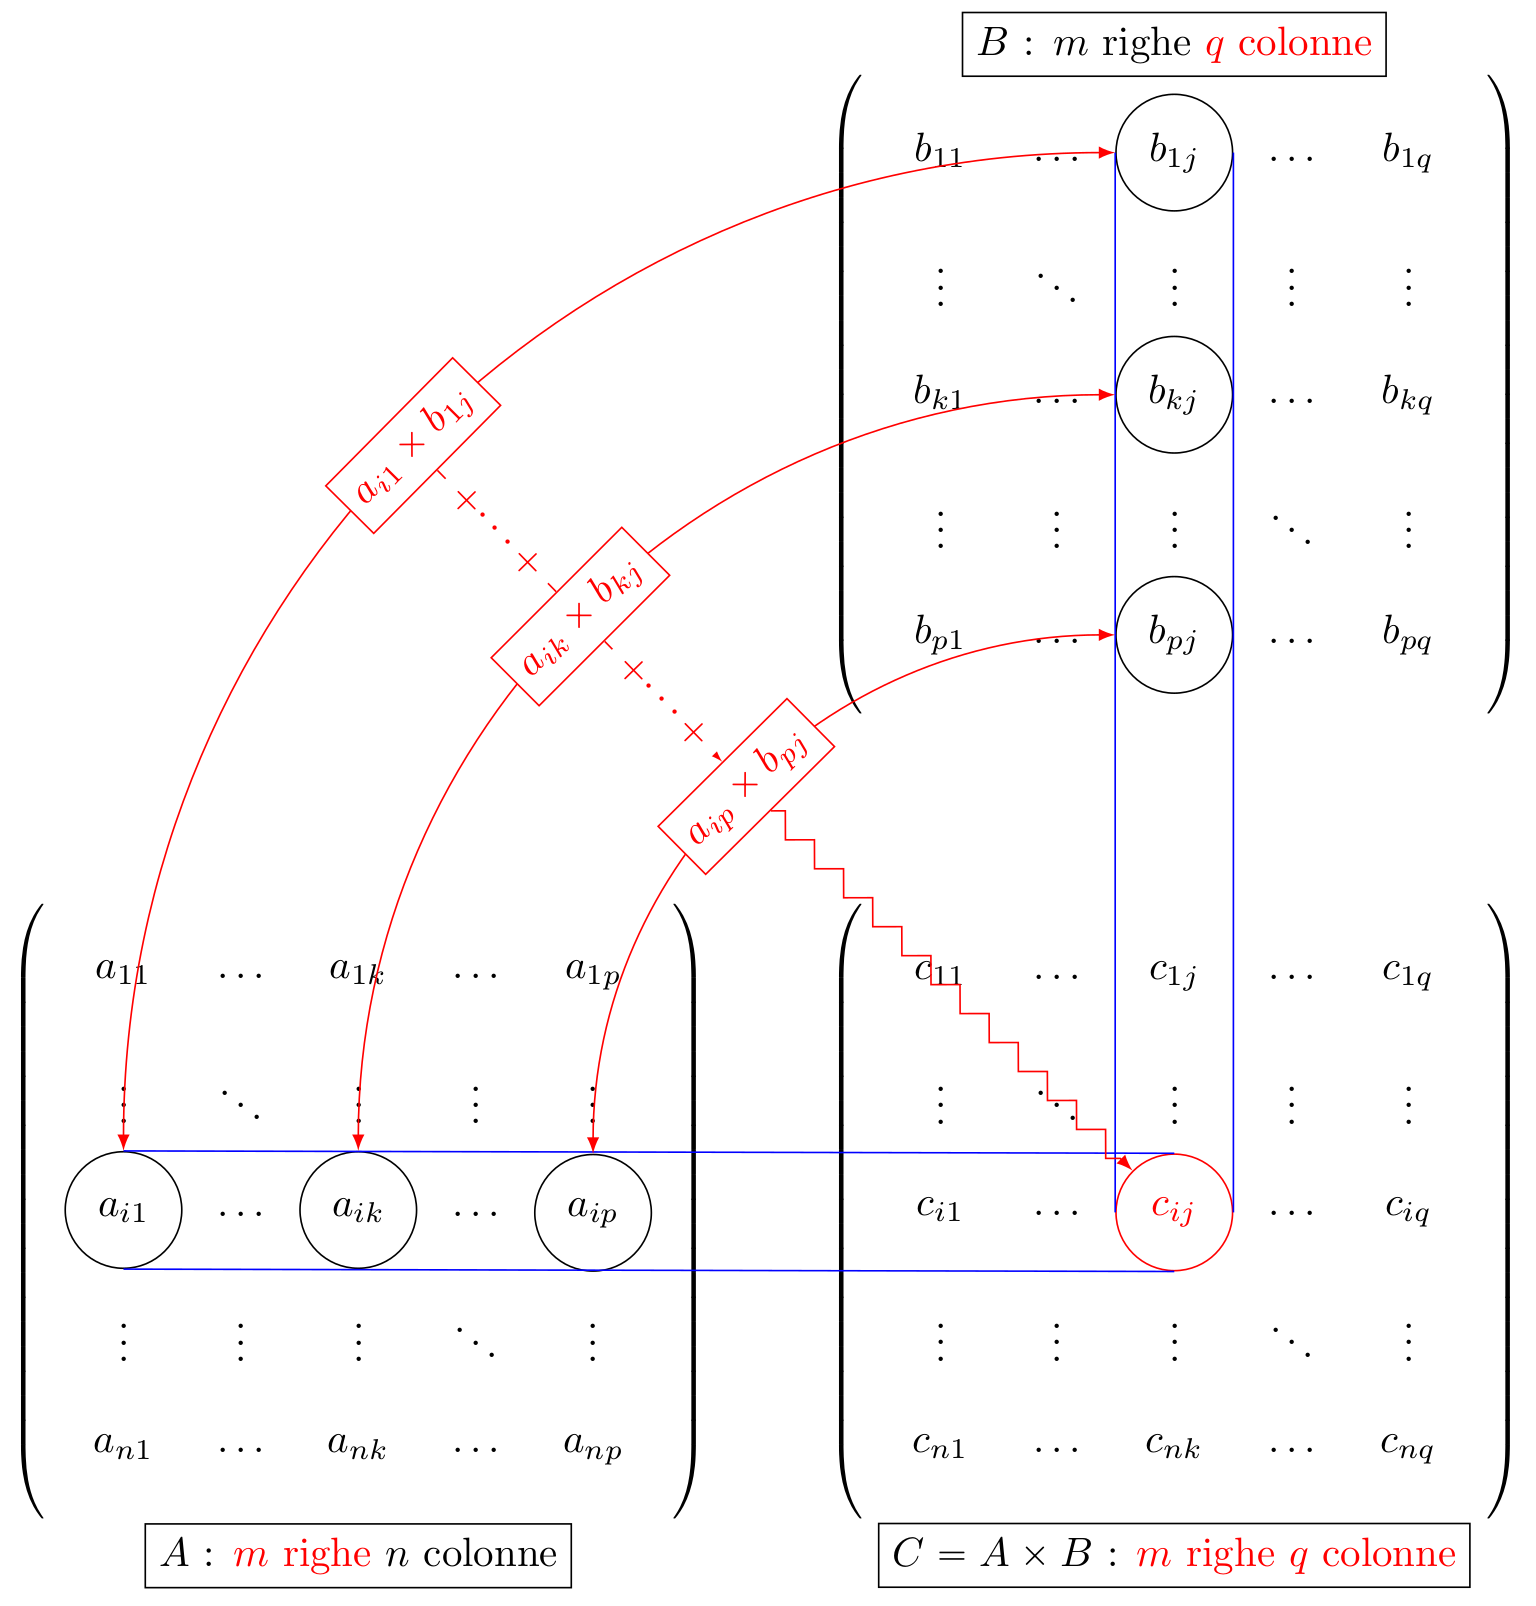
\includegraphics[width=0.6\linewidth]{images/matrMult.png}
    \caption{Illustrazione grafica per la moltiplicazione tra matrici}
    \label{fig:matrMult}
  \end{figure}
\end{Def}

\begin{SubDef}{Proprietà del prodotto tra matrici}
  Per il prodotto tra matrici vigono alcune proprietà:
  \begin{enumerate}
    \item Associativa: $(AB)C = A(BC)\quad\forall A\in\mathbb{R}^{m,n},
      B\in\mathbb{R}^{n,k},C\in\mathbb{R}^{k,q}$
    \item Distributiva del prodotto per la somma: $A(B+C) = AB+AC\quad\forall
      A\in\mathbb{R}^{m,n},B,C\in\mathbb{R}^{n,p}$
    \item $(\lambda A)B = \lambda(AB) = A(\lambda B)\quad\forall A\in\mathbb{R}^{m,n},
      B\in\mathbb{R}^{n,p}$
    \item Solo per le matrici quadrate: $IA = A = AI\quad\forall A\in\mathbb{R}^{n,n}$
  \end{enumerate}
\end{SubDef}
Si noti che per il prodotto $\exists A,B\suchthat AB=0 \notimplies A=O\lor B=O$. Si noti
anche che sempre per il prodotto, in generale $AB=AC\notimplies B=C$ con $A\neq O$.

\begin{Def}{Trasposto di una matrice}
  Data $A\in\mathbb{R}^{m,n}$ si dice trasposta di $A$ e si indica con $\transp A$ la matrice
  che si ottiene invertendo righe con colonne. Formalmente
  \begin{equation*}
    \text{Se}\; A=(a_{ij}),\; \transp A = (b_{ij})\implies b_{ij} = a_{ji}\quad\forall
    i=1,\ldots,m, j=1,\ldots,n
  \end{equation*}
\end{Def}

\begin{SubDef}{Proprietà del trasposto di una matrice}
  Il trasposto gode di alcune proprietà
  \begin{enumerate}
    \item $\transp(A+B) = \transp A+\transp b\quad\forall A,B\in\mathbb{R}^{m,n}$
    \item $\transp (\lambda A)=\lambda \transp A\forall\lambda\in\mathbb{R},
      A\in\mathbb{R}^{m,n}$
    \item $\transp{(AB)} = \transp B\transp A$
    \item Se $A\in GL(n,\mathbb{R})$ e $A^{-1}$ è la sua inversa, allora anche
      $\transp{A}\in GL(n,\mathbb{R})$ e si ha ${(\transp A)}^{-1} = \transp{(A^{-1})}$
      \begin{proof}
        Si deve dimostrare che
        \begin{equation*}
          \transp{(A^{-1})}\transp A = \transp{(AA^{-1})} = \transp I = I
        \end{equation*}
        e
        \begin{equation*}
          \transp A\transp{(A^{-1})} = \transp (A^{-1}A) = \transp I = I
        \end{equation*}
      \end{proof}
  \end{enumerate}
\end{SubDef}

\begin{Def}{Traccia di una matrice quadrata}\label{def:matrice_traccia}
  Sia $A\in\mathbb{R}^{n,n}$. Di definisce la sua traccia
  \begin{equation*}
    \tr(A)\bydef\sum_{i=1}^{n}a_{ii}
  \end{equation*}
\end{Def}

\begin{SubDef}{Proprietà della traccia}
  La traccia gode di alcune proprietà:
  \begin{enumerate}
    \item $\tr(A+B) = \tr(A) + \tr(B)\quad\forall A,B\in\mathbb{R}^{n,n}$
    \item $\tr(\lambda A) = \lambda\tr(A)\quad\forall\lambda\in\mathbb{R},
      A\in\mathbb{R}^{n,n}$
    \item $\tr(AB) = \tr(BA)\quad\forall A,B\in\mathbb{R}^{n,n}$
      \begin{proof}
        Siano $A=(a_{ij})$ e $B=(b_{ij})\in\mathbb{R}^{n,n}$. Allora $AB=(c_{ij})$. Per
        la~\autoref{def:matrice_prodotto}
        \begin{equation*}
          c_{ii} = \sum^{n}_{k=1} a_{ik}b_{ki}
        \end{equation*}
        Per la~\autoref{def:matrice_traccia}
        \begin{equation}\label{eq:matrice_traccia_3_dim_1}
          \tr(AB) = \sum^{n}_{i=1} c_{ii}= \sum^{n}_{i=1} \sum^{n}_{k=1} a_{ik}b_{ki}=
          \sum^{n}_{i,k=1} a_{ik}b_{ki}
        \end{equation}
        Sia $BA = (d_{ij})$, allora
        \begin{equation*}
          d_{ii} = \sum^{n}_{k=1} b_{ik}a_{ki}
        \end{equation*}
        Per la~\autoref{def:matrice_traccia}
        \begin{equation}\label{eq:matrice_traccia_3_dim_2}
          \tr(BA) = \sum^{n}_{i=1} d_{ii} = \sum^{n}_{i=1} \sum^{n}_{k=1} b_{ik}a_{ki} =
          \sum^{n}_{i,k=1} b_{ik}a_{ki}
        \end{equation}
        Dato che in $\mathbb{R}$ il prodotto è commutativo e che sia $i$ che $k$, sia in
        \eqref{eq:matrice_traccia_3_dim_1} e \eqref{eq:matrice_traccia_3_dim_2} variano
        da $1$ a $n$, si può affermare che
        \begin{equation*}
          \sum^{n}_{i,k=1} a_{ik}b_{ki} = \sum^{n}_{i,k} b_{ik}a_{ki}
        \end{equation*}
      \end{proof}
    \item $\tr(\transp A) = \tr(A)\quad\forall A\in\mathbb{R}^{n,n}$
  \end{enumerate}
\end{SubDef}

%!TEX ROOT=geometria1.tex

\section{Equazioni e sistemi lineari}%
\label{sec:equazioni_e_sistemi_lineari}

\subsection{Equazioni lineari}%
\label{sub:equazioni_lineari}

\begin{Def}{Equazione lineare}
  Un'equazione lineare nelle incognite $x_1,x_2,\ldots,x_n$ è un'espressione del tipo
  \begin{equation}\label{eq:lineare_equazione}
    a_1x_1+a_2x_2+\cdots+a_n x_n=b
  \end{equation}
  dove $a,b\in\mathbb{R}, i=1,\ldots,n$.\\
  $a_i$ sono detti coefficienti, $b$ è detto termine noto.\\
  Scritta in forma matriciale
  \begin{equation*}
    \begin{pmatrix}
      a_1&a_2&a_3&\cdots&a_n
    \end{pmatrix}
    \begin{pmatrix}
      x_1\\x_2\\\vdots\\x_n
    \end{pmatrix}
    = b
  \end{equation*}
\end{Def}

\begin{Def}{Soluzione dell'equazione lineare}
  Una soluzione dell'equazione lineare~\eqref{eq:lineare_equazione} è una $n$-upla di
  numeri reali
  $(\widetilde{x_1},\widetilde{x_2},\ldots,\widetilde{x_n})$ che sostituiti
  nell'equazione, la verifica.
\end{Def}

\begin{Def}{Equazione lineare omogenea}
  L'equazione~\eqref{eq:lineare_equazione} si dice omogenea se $b=0$.
\end{Def}

\begin{SubDef}{Soluzione particolare}
  La $n$-upla $(0,0,\ldots,0)$ è soluzione dell'equazione omogenea.
\end{SubDef}

\begin{SubDef}{Soluzione particolare}\label{def:lineare_equazione_soluzione_particolare_2}
  Se $(\tilde{x_1},\ldots,\tilde{x_n})$ è soluzione, lo è anche
  $(t\tilde{x_1},\ldots,t\tilde{x_n})$.
\end{SubDef}

\subsection{Sistemi lineari}%
\label{sub:sistemi_lineari}

\begin{Def}{Sistema lineare}
  Un sistema lineare di $m$ equazioni e $n$ incognite $x_1,\ldots,x_n$ è un instieme di
  equazioni lineari del tipo
  \begin{equation}\label{eq:lineare_sistema}
    \begin{cases}
      a_{11}x_1+\cdots+a_{1m}x_n &= b_1\\
      \vdots &= \vdots\\
      a_{m1}x_1+\cdots+a_{mn}x_n &= b_m
    \end{cases}
  \end{equation}
  $a_{ij}$ si dicono coefficienti (con $i=1,\ldots,n,\;j=1,\ldots,m$).\\
  $b_{i}$ si dicono termini noti.\\
  Scritto in forma matriciale
  \begin{equation*}
    AX=B
  \end{equation*}
  in cui
  \begin{alignat*}{2}
    A &=
    \begin{pmatrix}
      a_{11} & \cdots & a_{1m}\\
      \vdots & \ddots & \vdots\\
      a_{m1} & \cdots & a_{mn}
    \end{pmatrix}\in\mathbb{R}^{m,n} &\qquad &\text{Matrice dei coefficienti}\\
    X &=
    \begin{pmatrix}
      x_1\\\vdots\\x_n
    \end{pmatrix}\in\mathbb{R}^{n,1} & B &=
    \begin{pmatrix}
      b_1\\\vdots\\b_m
    \end{pmatrix}\in\mathbb{R}^{m,1}
  \end{alignat*}
\end{Def}

\begin{Def}{Matrice completa}
  Si definisce matrice completa
  \begin{equation*}
    (A\vert B)=
    \begin{pmatrix}[ccc|c]
      a_{11} & \cdots & a_{1m} & b_1\\
      \vdots & \ddots & \vdots & \vdots\\
      a_{m1} & \cdots & a_{mn} & b_m
    \end{pmatrix}
  \end{equation*}
  Ciascuna riga si indica con $R_i$.
\end{Def}

\begin{Def}{Sistema lineare omogeneo}
  Un sistema lineare è omogeneo se $b_j=0\;\forall j=1,\ldots,m$, ovvero
  \begin{equation*}
    AX=O
  \end{equation*}
\end{Def}

\begin{Def}{Soluzione del sistema lineare}
  Soluzione del sistema lineare~\eqref{eq:lineare_sistema} è una $n$-upla di numeri
  reali $(\widetilde{x_1},\ldots,\widetilde{x_n})$ che sostituia nelle ingognite
  verifica tutte le equazioni.
\end{Def}

\begin{SubDef}{Soluzioni di un sistema omogeneo}
  Se un sistema lineare è omogeneo, allora $(0,\ldots,0)$ è una sua soluzione. Si
  conclude quindi che un sistema lineare omogeneo è sempre compatibile.
\end{SubDef}

\begin{Def}{Sistema compatibile}
  Un sistema lineare si dice compatibile se ammette soluzioni, incompatibile altrimenti.
\end{Def}

\begin{Def}{Sistema equivalente}
  Un sistema si dice equivalente ad un altro se ammette le stesse soluzioni.
\end{Def}

\subsubsection{Metodo di riduzione di Gauss}%
\label{ssub:metodo_di_riduzione_di_gauss}

Il metodo di riduzione di Gauss permette di semplificare un sistema lineare in uno
equivalente.

\begin{Thm}{Operazioni elementari di riduzione per righe}
  Eseguendo un numero finito di volte le tre operazioni
  \begin{enumerate}
    \item\label{thm:lineare_riduzione_1} Scambiare due equazioni
    \item\label{thm:lineare_riduzione_2} Moltiplicare per un numero reale diverso da
      $0$
    \item\label{thm:lineare_riduzione_3} Sostituire ad un'equazione la somma di se
      stessa con un'altra equazione moltiplicata per un qualsiasi numero reale
  \end{enumerate}
  si ottiene un sistema lineare equivalente.
\end{Thm}

\begin{proof}
  Dimostrare~\ref{thm:lineare_riduzione_1} è ovvio, in quanto le equazioni non si
  modificano.\\
  Il punto~\ref{thm:lineare_riduzione_2} invece deve essere dimostrato che se una
  $n$-upla è soluzione di un sistema, lo è anche dell'altro e viceversa. Si ha quindi
  \begin{equation*}
    \begin{cases}
      a_{11}x_1+\ldots a_{1n}x_n &= b_1\\
      \vdots &= \vdots\\
      a_{m1}x_1+\ldots a_{mn}x_m &= b_m
    \end{cases} \implies
    \begin{cases}
      \lambda(a_{11}x_1+\ldots a_{1n}x_n) &= \lambda b_1\\
      \vdots &= \vdots\\
      a_{m1}x_1+\ldots a_{mn}x_m &= b_m
    \end{cases}
  \end{equation*}
  Per~\autoref{def:lineare_equazione_soluzione_particolare_2} si ha che la seconda
  equazione ha le stesse soluzioni della prima.
  \begin{equation*}
    \begin{cases}
      \lambda(a_{11}x_1+\ldots a_{1n}x_n) &= \lambda b_1\\
      \vdots &= \vdots\\
      a_{m1}x_1+\ldots a_{mn}x_m &= b_m
    \end{cases} \implies
    \begin{cases}
      a_{11}x_1+\ldots a_{1n}x_n &= b_1\\
      \vdots &= \vdots\\
      a_{m1}x_1+\ldots a_{mn}x_m &= b_m
    \end{cases}
  \end{equation*}
  dividendo per $\lambda\neq0$.
  Per~\autoref{def:lineare_equazione_soluzione_particolare_2} si ha che hanno le stesse
  soluzioni.\\
  Per il punto~\ref{thm:lineare_riduzione_3} si procede analogamente al
  punto~\ref{thm:lineare_riduzione_2}.
\end{proof}

Dal punto di vista matriciale, le trasformazioni si applicano nei seguenti modi
\begin{align*}
  R_i &\leftrightarrow R_j\\
  R_i &\leftrightarrow \lambda R_i\quad\lambda\neq0\\
  R_i &\leftrightarrow R_i+\lambda R_j\quad\lambda\in\mathbb{R},\;j\neq i
\end{align*}
Eseguire queste operazioni un numero finito di volte significa trasformare $(A\vert B)$
in $(\widetilde{A}\vert\widetilde{B})$ in modo che ogni riga di $\widetilde{A}$ non
nulla esista un elemento non nullo sotto il quale sono tutti $0$.

\begin{Def}{Sistema ridotto}
  Un sistema lineare è ridotto se è ridotta $A$.
\end{Def}

\begin{Thm}{Teorema di Rouché-Capelli}\label{thm:lineare_rouche-capelli}
  Un sistema lineare di $m$ equazioni e $n$ incognite
  \begin{equation*}
    AX = B
  \end{equation*}
  è compatibile se e solo se
  \begin{equation*}
    \rank(A) = \rank(A\vert B)
  \end{equation*}
\end{Thm}

In particolare si ha che se $\rank(A)=\rank(A\vert B)=n$ la soluzione è unica. Se invece
$\rank(A)=\rank(B)=k<n$ ci sono infinite soluzioni che dipendono da $n-k$ variabili.
Quindi ci sono $\infty^{n-k}$ soluzioni.

\begin{SubThm}{Teorema di Rouché-Capelli per un sistema lineare omogeneo}
  Un sistema lineare omogeneo di $m$ equazioni e $n$ incognite
  \begin{equation*}
    AX = O
  \end{equation*}
  è sempre compatibile. Se
  \begin{equation*}
    \rank(A) = n
  \end{equation*}
  esiste un'unica soluzione che è quella nulla. Se
  \begin{equation*}
    \rank(A) = k < n
  \end{equation*}
  il sistema ammette $\infty^{n-k}$ soluzioni.
\end{SubThm}

Si noti che se $AX=B$ ha un'unica soluzione e utilizzando il metodo di riduzione di
Gauss-Jordan si può arrivare ad una matrice ridotta a scala del tipo
\begin{equation*}
  \begin{pmatrix}[cccc|c]
    1 & 0 & \cdots & 0 & \widetilde{b_1}\\
    0 & 1 & \cdots & \vdots & \vdots\\
    \vdots & \cdots & \ddots & \vdots & \vdots\\
    0 & \cdots & \cdots & 1 & \widetilde{b_n}
  \end{pmatrix}
\end{equation*}
in cui si ha che $A=I$.


\subsection{Equazioni matriciali}%
\label{sub:equazioni_matriciali}

\begin{Def}{Equazione matriciale}
  Un'equazione matriciale è un'equazione del tipo
  \begin{equation*}
    AX = B
  \end{equation*}
  con $A\in\mathbb{R}^{m,n}$, $X\in\mathbb{R}^{n,p}$, $B\in\mathbb{R}^{m,p}$.
\end{Def}

\begin{SubDef}{Casi particolari}
  Se $p=1$, si ha un sistema lineare.\\
  Se $AX=I$, si ha che $X$ è l'inversa di $A$.\\
  Se si ha $YC=D$, si può ricondurre in modo che $\transp(YC)=\transp C\iff\transp
  C\transp Y = \transp D$.
\end{SubDef}

Se ad esempio si pensa di scrivere $X$ come matrice colonna di $n$-uple, del tipo
\begin{equation*}
  X =
  \begin{pmatrix}
    X_1\\
    \vdots\\
    X_n
  \end{pmatrix}
\end{equation*}
e la stessa cosa per $B$
\begin{equation*}
  B =
  \begin{pmatrix}
    B_1\\
    \vdots\\
    B_n
  \end{pmatrix}
\end{equation*}
si può scrivere l'equazione matriciale come sistema
\begin{equation}\label{eq:lineare_matriciale}
  AX = B \iff
    \begin{cases}
      a_{11}x_1 + \cdots + a_{1m}x_1 &= B_1\\
      \vdots & \vdots\\
      a_{n1}x_1 + \cdots + a_{nm}x_n &= B_n
    \end{cases}
\end{equation}
Si può notare come~\eqref{eq:lineare_matriciale} sia equivalente ad un sistema lineare
di $pn$  incognite $x_{ij}$.

%!TEX ROOT=geometria1.tex

\section{Spazio vettoriale}%
\label{sec:spazio_vettoriale}

\begin{Def}{Spazio vettoriale}
  Un insieme $V$ si definisce spazio vettoriale sul campo $\mathbb{K}$ se sono definite
  su $V$ due operazioni
  \begin{enumerate}
    \item \textbf{Somma} definita come
      \begin{align*}
        +:\,&V\times V\to V\\
            &(\vec{x},\vec{y})\mapsto\vec{x}+\vec{y}
      \end{align*}
      rispetto alla quale $(V,\,+)$ ha la struttura di gruppo commutativo. Ovvero
      \begin{enumerate}
        \item $\vec{x}+\vec{y} = \vec{y}+\vec{x}$
        \item $(\vec{x}+\vec{y})+\vec{z} = \vec{x} + (\vec{y}+\vec{z})$
        \item $\exists\vec{o}\in V\suchthat \vec{x}+\vec{o}=\vec{x}$ e si definisce
          $\vec{o}$ vettore nullo.
        \item $\forall\vec{x}\in V\,\exists\vec{x}\in
          V\suchthat\vec{x}+(-\vec{x})=\vec{o}$ e si definisce opposto.
      \end{enumerate}
    \item \textbf{Prodotto} definito per uno scalare
      \begin{align*}
        &\mathbb{K}\times V\to V\\
        &(\lambda,\vec{x})\mapsto \lambda\vec{x}
      \end{align*}
      e si ha che
      \begin{enumerate}
        \item $\lambda(\vec{x}+\vec{y}) = \lambda\vec{x}+\lambda\vec{y}$
        \item $(\lambda+\mu)\vec{x} = \lambda\vec{x}+\mu\vec{x}$
        \item $(\lambda\mu)\vec{x} = \lambda(\mu\vec{x})$
        \item $1\vec{x} = \vec{x}$
      \end{enumerate}
  \end{enumerate}
\end{Def}

\begin{Def}{Eleementi dello spazio}
  Gli elementi di $V$ sono detti vettori, quelli di $\mathbb{K}$ scalari.
\end{Def}

\begin{Def}{Campo}
  Un campo è un insieme i cui elementi sono detti numeri, che contiene $0$ e $1$ e ha
  due operazioni $+$ e $\cdot$ che verificano
  \begin{multicols}{2}
    \begin{enumerate}
      \item $\alpha+\beta = \beta+\alpha$
      \item $\alpha+(\beta+\gamma) = (\alpha+\beta)+\gamma$
      \item $\alpha+0 = \alpha$
      \item $\alpha+(-\alpha)=0$
      \columnbreak%
      \item $\alpha\beta = \beta\alpha$
      \item $(\alpha\beta)\gamma = \alpha(\beta\gamma)$
      \item $1\alpha = \alpha$
      \item $\alpha\alpha^{-1}=1$ se $\alpha\neq0$
      \item $(\alpha+\beta)\gamma = \alpha\gamma+\beta\gamma$
    \end{enumerate}
  \end{multicols}
\end{Def}

\subsection{Spazi particolari}%
\label{sub:spazi_particolari}

In generale $\mathbb{R}^n$ è uno spazio vettoriale, così come anche in generale
$\mathbb{K}^n$. Infatti si ha che
\begin{equation*}
  (x_1,\ldots,x_2)+(y_1,\ldots,y_n) = (x_1+y_1,\ldots,x_n+y_n)
\end{equation*}
e
\begin{equation*}
  \lambda(x_1,\ldots,x_n) = (\lambda x_1,\ldots,\lambda x_n)
\end{equation*}
In generale anche $\mathbb{K}^{m,n}$ è uno spazio vettoriale (e quindi anche
$\mathbb{R}^{m,n}$).\\
Il più piccolo spazio vettoriale è quello composto dal solo vettore nullo, ovvero
$\{\vec{o}\}$.\
Un caso particolare è lo spazio dei polinomi reali in $x$, denotato come $\mathbb{R}[x]$
che è
\begin{equation*}
  \mathbb{R}[x]\bydef \left\{ a_0+a_1x+\cdots+a_n x^n\Setsuchthat
  n\in\mathbb{N},\,a_i\in\mathbb{R},\,i=0,\ldots,n \right\}
\end{equation*}
È anche interessante il caso in cui si consideri l'insieme
\begin{equation*}
  \mathscr{F} = \left\{ f:\,\mathbb{R}\to\mathbb{R}\qq{funzione} \right\}
\end{equation*}
in quanto anche questo è uno spazio vettoriale infatti
\begin{equation*}
  (f+g)(x)\bydef f(x)+g(x)
\end{equation*}
e
\begin{equation*}
  (\lambda f)(x)\bydef \lambda f(x)
\end{equation*}

\subsection{Proprietà formali}%
\label{sub:proprieta_formali}

In un campo vettoriale su $\mathbb{K}$ valgono le seguenti proprietà
\begin{enumerate}
  \item Vettore nullo unico
    \begin{proof}
      Supponiamo per assurdo che esistano $\vec{o}$ e $\vec{o'}$ nulli in modo che
      $\vec{o}\neq\vec{o'}$. Allora si ha $\vec{o}=\vec{o}+\vec{o'}$ sfruttando il fatto
      che $\vec{o'}$ è un vettore nullo. Analogamente si ha che
      $\vec{o'}=\vec{o'}+\vec{o}$. Da queste due relazioni si deduce che
      $\vec{o'}=\vec{o}$ che va contro l'ipotesi iniziale.
    \end{proof}
  \item Opposto unico
    \begin{proof}
      Supponiamo per assurdo che esistano $\vec{x_1}\neq\vec{x_2}$ oposti di $\vec{x}$.
      Allora possiamo scrivere $(\vec{x}+\vec{x_1})+\vec{x_2} =
      \vec{o}+\vec{x_2}=\vec{x_2}$. Analogamente si ha che
      $(\vec{x}+\vec{x_1})+\vec{x_2}=\vec{x}+(\vec{x_2}+\vec{x_1})=(\vec{x}+\vec{x_2})
      +\vec{x_1}=\vec{o}+\vec{x_1}=\vec{x_1}$. Si deduce quindi che
      $\vec{x_1}=\vec{x_2}$ ma per ipotesi questo non può essere.
    \end{proof}
  \item Se per $\vec{x}$, $\vec{y}$, $\vec{z}$ si ha $\vec{x}+\vec{y}=\vec{x}+\vec{z}$
    allora $\vec{y}=\vec{z}$
    \begin{proof}
      La dimostrazione segue direttamente dalla seconda proprietà, infatti si può
      aggiungere $-\vec{x}$ ad entrambi i membri e ottenere
      $\vec{x}+\vec{y}-\vec{x}=\vec{x}+\vec{z}-\vec{x}$. Si ottiene
      $\vec{o}+\vec{y}=\vec{z}+\vec{o}$ e infine $\vec{y}=\vec{z}$.
    \end{proof}
  \item Solo su $\mathbb{R}$ vale che $\lambda\vec{x}=\vec{o}$ con
    $\lambda\in\mathbb{R}$ allora $\lambda=0\lor\vec{x}=\vec{o}$
    \begin{proof}
      Essendo una biimplicazione, bisogna dimostrare entrambi i versi. Dimostriamo
      $\Leftarrow$. Possiamo provare che $0\vec{x}\vec{o}$ e $\lambda\vec{o}=\vec{o}$.
      Per il primo caso si può dire che $0\vec{x}=(0+0)\vec{x}=0\vec{x}+0\vec{x}$. Per
      il punto precedente, abbiamo che $o\vec{x}=o\vec{x}+o\vec{x}$ e semplificando si
      ottiene $\vec{o}=o\vec{x}$. Il secondo caso si dimostra analogamente
      $\lambda\vec{o}=\lambda(\vec{o}+\vec{o})=\lambda\vec{o}+\lambda\vec{o}$. Per il
      punto precedente $\lambda\vec{o}=\vec{o}\lambda+\lambda\vec{o}$, semplificando
      $\vec{0}=\lambda\vec{o}$.\\
      L'altro vers ($\Rightarrow$) dice che $\lambda\vec{x}=\vec{o}$. Se $\lambda=0$ è
      immediato. Se $\lambda\neq0$, sicuramente $\exists\lambda^{-1}$. Possiamo allora
      scrivere $\vec{o}=\lambda^{-1}\vec{o}=\lambda^{-1}(\lambda\vec{o}\vec{x})=
      (\lambda^{-1}\lambda)\vec{x}=\vec{x}$.
    \end{proof}
  \item $(-1)\vec{x} = -\vec{x}$
    \begin{proof}
      Si ha che $\vec{x}+(-1)\vec{x}=1\vec{x}+(-1)\vec{x}=(1-1)\vec{x}=\vec{o}$.
    \end{proof}
\end{enumerate}

\subsection{Sottoinsiemi di spazi vettoriali}%
\label{sub:sottoinsiemi_di_spazi_vettoriali}

\begin{Def}{Sottospazio vettoriale}
  Sia $V$ uno spazio vettoriale su $\mathbb{K}$. Un sottoinsieme $W$ di $V$ è un
  sottospazio vettoriale di $V$ se $W$ è uno spazio vettoriale rispetto alle stesse
  operazioni di $V$, ovvero rispetto alla somma e al prodotto per scalari. Formalmente
  se vale
  \begin{equation*}
    \forall\lambda,\mu\in\mathbb{K}\;\forall\vec{x},\vec{y}\in W\quad
    \lambda\vec{x}+\mu\vec{y}\in W
  \end{equation*}
\end{Def}
Si noti che $(W,+)$ è un sottgruppo di $V$ rispetto alla somma. Si noti anche che il
vettore nullo di $V$ appartiene ad ogni sottospazio vettoriale $W$ di $V$, infatti
$\lambda\vec{x}\in W\quad\lambda=0\implies\lambda\vec{x}=\vec{o}\in W$.

\begin{SubDef}{Sottospazi impropri}
  Ogni spazio vettoriale ha almeno due sottospazi vettoriali: se stesso e $\{\vec{o}\}$.
\end{SubDef}

Si noti anche che se $W$ è un sottospazio vettoriale, $\vec{x}\in W\implies-\vec{x}\in
W$.

\subsubsection{Esempio fondamentale di sottospazio vettoriale}%
\label{ssub:esempio_fondamentale_di_sottospazio_vettoriale}

Si prenda l'insieme delle soluzioni di un sistema lineare omogeneo di $m$ equazioni in
$n$ incognite. L'insieme è un sottospazio vettoriale di $\mathbb{R}^n$. In generale
l'insieme di soluzioni di $AX=B$ è un sottospazio vettoriale di $\mathbb{R}^n$ se e solo
se il sistema è omogeneo.

\begin{Def}{Nullspace}
  Sia $AX=O$ un sistema lineare omogeneo con $A\in\mathbb{R}^{m,n}$ e
  $X=
  \begin{pmatrix}
    X_1\\\vdots\\X_n
  \end{pmatrix}\in\mathbb{R}^{n,1}$. Allora
  \begin{equation*}
    N(A)\bydef \left\{ X\in\mathbb{R}^{n,1}\Setsuchthat AX = O
    \right\}\subseteq\mathbb{R}^n
  \end{equation*}
  si definisce \textbf{nullspace} di $A$ che contiene l'insieme delle soluzioni.
\end{Def}

Il nullspace è uno sottospazio vettoriale in quanto
$\forall\lambda,\mu\in\mathbb{R}\;\forall X,Y\in N(A)\quad \lambda X+\mu Y\in N(A)$.
Infatti si ha che $A(\lambda X+\mu Y) = O = \lambda AX+\mu (AY)$ in quanto sia $X$ che
$Y$ sono soluzioni.

\subsubsection{Esempi di sottospazi vettoriali nello spazio delle matrici}%
\label{sub:esempi_di_sottospazi_vettoriali_nello_spazio_dell_matrici}

\begin{Def}{Insieme delle matrici diagonali}
  \begin{equation*}
    \mathscr{D}\left( \mathbb{R}^{n,n} \right) \bydef \left\{ D =
      \begin{pmatrix}
        d_1 & \cdots & 0\\
        0 & \ddots & \vdots\\
        0 & 0 & d_n
      \end{pmatrix}\in\mathbb{R}^{n,n}
      \Setsuchthat d_i\in\mathbb{R}^{n,n}
    \right\}
  \end{equation*}
  È uno sottospazio vettoriale in quanto combinazioni lineari di matrici diagonali, sono
  ancora matrici diagonali.
\end{Def}

\begin{Def}{Insieme delle matrici triangolari superiori e inferiori}
    \begin{equation*}
      \tau \left( \mathbb{R}^{n,n} \right)\bydef \left\{
        \begin{pmatrix}
          a_{11} & \cdots & \cdots & a_{1n}\\
          0 & a_{22} & \cdots & a_{2n}\\
          \vdots & \cdots & \ddots & \vdots\\
          0 & \cdots & 0 & a_{nn}
        \end{pmatrix}\in\mathbb{R}^{n,n}
        \Setsuchthat a_{ij}\in\mathbb{R}
      \right\}
    \end{equation*}
    e
    \begin{equation*}
      \tau \left( \mathbb{R}^{n,n} \right)\bydef \left\{
        \begin{pmatrix}
          a_{11} & 0 & \cdots & 0\\
          \vdots & a_{22} & 0 & \vdots\\
          \vdots & \cdots & \ddots & \vdots\\
          a_{n1} & \cdots & \cdots & a_{nn}
        \end{pmatrix}\in\mathbb{R}^{n,n}
        \Setsuchthat a_{ij}\in\mathbb{R}
      \right\}
    \end{equation*}
    sono sottospazi vettoriali di $\mathbb{R}^{n,n}$.
\end{Def}

\begin{Def}{Insieme delle matrici simmetriche}
  \begin{equation*}
    \mathscr{S}\left( \mathbb{R}^{n,n} \right)\bydef \left\{A\in\mathbb{R}^{n,n}\Setsuchthat
    \transp A = A\right\}
  \end{equation*}
  è uno sottospazio vettoriale di $\mathbb{R}^{n,n}$.
\end{Def}

\begin{Def}{Insieme delle matrici antisimmetriche}
  \begin{equation*}
    \mathscr{S}\left( \mathbb{R}^{n,n} \right)\bydef \left\{A\in\mathbb{R}^{n,n}\Setsuchthat
    \transp A = -A\right\}
  \end{equation*}
  è un sottospazio vettoriale di $\mathbb{R}^{n,n}$.
\end{Def}

\begin{Def}{Insieme delle matrici ortogonali reali}
  \begin{equation*}
    \mathscr{O}(n,\mathbb{R})\bydef \left\{ A\in\mathbb{R}^{n,n}\Setsuchthat A\transp A
    = I = \transp A A\right\}
  \end{equation*}
  \textbf{non} è uno sottospazio vettoriale di $\mathbb{R}^{n,n}$ in quanto $O\notin
  O(n,\mathbb{R})$.
\end{Def}

\subsection{Combinazioni lineari}%
\label{sub:combinazioni_lineari}

\begin{Def}{Combinazione lineare}
  Dati $l$ vettori $\vec{v_1},\ldots,\vec{v_l}$ di uno spazio vettoriale $V$ su
  $\mathbb{K}$, si dice che un vettore $\vec{x}$ è una combinazione lineare dei vettori
  $\vec{v_1},\ldots,\vec{v_l}$ se esistono $x_1,\ldots,x_l\in\mathbb{K}$ tali che
  $\vec{x}=x_1\vec{v_1}+\cdots+x_l\vec{v_l}$. $x_i$ si dice coefficiente.
\end{Def}

\begin{Def}{Insieme delle combinazioni lineari}
  Fissando i vettori $\vec{v_1},\ldots,\vec{v_2}$, si definisce
  \begin{equation*}
    \mathscr{L}(\vec{v_1},\ldots,\vec{v_l})\bydef \left\{
    x_1\vec{v_1}+\cdots+x_l\vec{v_l} \Setsuchthat x_i\in\mathbb{K},\;i=1,\ldots,l \right\}
  \end{equation*}
\end{Def}

\begin{Def}{Sistema di generatori di $\mathscr{L}(\vec{v_1},\ldots,\vec{v_l})$}
  Il sistema di generatori è l'insieme $\{x_1\vec{v_1},\ldots,x_l\vec{v_l}\}$.
\end{Def}

\begin{Thm}{Sottospazio delle combinazioni lineari}
  $\mathscr{L}(\vec{v_1},\ldots,\vec{v_l})$ è un sottospazio vettoriale di $V$ ed è il
  più piccolo sottospazio vettoriale di $V$ a contenere i vettori
  $\vec{v_1},\ldots,\vec{v_l}$.
\end{Thm}

\begin{Def}{Sistema di generatori di un sottospazio}
  Siano $\vec{v_1},\ldots,\vec{v_l}$ vettori di $V$. Si dice che un sottospazio
  vettoriale $W$ di $V$ ha come sistema di generatori $\{\vec{v_1},\ldots,\vec{v_l}\}$
  se $W=\mathscr{L}(\vec{v_1},\ldots,\vec{v_l})$.
\end{Def}

\begin{Thm}{Modifiche ai generatori}
  Detto $W=\mathscr{L}(\vec{v_1},\ldots,\vec{v_l})$, si possono aggiungere o sostituire
  più generatori di $W$ con loro combinazioni lineari.
\end{Thm}

Come conseguenza di questo teorema si ha che $W=\mathscr{L}(\vec{v_1},\ldots,\vec{v_l})$
ha infiniti sistemi generatori.

\begin{Def}{Spazi finitiamente generati}
  Uno spazio vettoriale $V$ si dice finitamente generato se esistono $l$ vettori
  $\vec{v_1},\ldots,\vec{v_l}$ di $V$ tali che $V=\mathscr{L}(\vec{v_1},\ldots,\vec{v_l}
  )$.
\end{Def}

\begin{Def}{Sottospazi finitiamente generati}
  Un sottospazio vettoriale $W$ si dice finitamente generato se esistono $l$ vettori
  $\vec{v_1},\ldots,\vec{v_l}$ di $W$ tali che $W=\mathscr{L}(\vec{v_1},\ldots,\vec{v_l}
  )$.
\end{Def}

\subsubsection{Esempi di spazi finitamente generati}%
\label{ssub:esempi_di_spazi_finitamente_generati}

$\mathbb{R}^n$ è finitamente generato, in quanto possiamo definire
$\vec{e_1}=(1,0,\ldots,0)$, $\vec{e_i}=(0,\ldots,1,\ldots,0)$ dove l'$1$ è all'$i$-esimo
posto e $\vec{e_n}=(0,\ldots,1)$. In questo modo una qualsiasi $n$-upla la si può
scrivere come $(x_1,\ldots,x_n)=x_1\vec{e_1}+\cdots+x_n\vec{e_n}$.\\
Analogamente anche $\mathbb{R}^{m,n}$ è finitamente generato, creando delle matrici
nello stesso modo.

\subsubsection{Dipendenza lineare}%
\label{sub:dipendenza_lineare}

\begin{Def}{Vettori linearmente indipendenti}
  Dati $l$ vettori $\vec{v_1},\ldots,\vec{v_l}$ di $V$ su $\mathbb{K}$, si dicono
  linearmente indipendenti se l'unica loro combinazioni lineare uguale a $\vec{o}$ è
  quella che ha coefficienti tutti nulli.
\end{Def}

\begin{SubDef}{Insieme libero}
  L'insieme di vettori linearmente indipendenti è un insieme libero.
\end{SubDef}

\begin{Def}{Vettori linearmente dipendenti}
  Dati $l$ vettori $\vec{v_1},\ldots,\vec{v_l}$ di $V$ su $\mathbb{K}$, si dicono
  linearmente dipendenti se esiste almeno una combinazione lineare uguale a $\vec{o}$ a
  coefficienti non tutti nulli.
\end{Def}

\begin{Thm}{Dipendenza lineare e combinazioni lineari}
  Dati $l$ vettori $\vec{v_1},\ldots,\vec{v_l}$ di $V$ su $\mathbb{K}$ essi sono
  linearmente dipendenti se e solo se uno è combinazione lineare degli altri.
\end{Thm}

\begin{proof}
  Essendo un se e solo se, si devono dimostrare entrambe le implicazioni. Dimostrando
  $\Rightarrow$, si può dire per ipotesi che i vettori sono linearmente indipendenti, e
  quindi
  \begin{equation*}
    \exists x_1\vec{v_1}+\cdots+x_l\vec{v_l}=\vec{o}\qq{con} x_1\neq0
  \end{equation*}
  Isolando $\vec{v_1}$ si dimostra
  \begin{equation*}
    \vec{v_1}= - \frac{x_2}{x_1}\vec{v_1}-\cdots-\frac{x_l}{x_1}\vec{v_l}
  \end{equation*}
  L'altra implicazione ($\Leftarrow$) si dimostra anlogamente. Per ipotesi se
  \begin{equation*}
    \vec{v_i}=\lambda_1\vec{v_1}+\cdots+\lambda_{i-1}\vec{v_{i-1}}+
    \lambda_{i+1}\vec{v_{i+1}}+\cdots+\lambda_l\vec{v_l}
  \end{equation*}
  allora
  \begin{equation*}
    \vec{o} =
    \lambda_1\vec{v_1}+\cdots\lambda_{i-1}\vec{v_i-1}-\vec{v_i}+\lambda_{i+1}\vec{v_i+1}
    +\cdots+\lambda_l\vec{v_l}
  \end{equation*}
\end{proof}

\subsection{Base di uno spazio vettoriale}%
\label{sub:base_di_uno_spazio_vettoriale}

\begin{Def}{Base}
  Un insieme finito e ordinato di $V$ denotato con
  $\mathscr{B}(\vec{v_1},\ldots,\vec{v_n})$ è detto base di $V$ se è insieme libero e un
  sistema di generatori.
\end{Def}

\begin{SubDef}{Basi canoniche o standard}
  In $\mathbb{R}^n$,
  \begin{equation*}
    \mathscr{B}\bigl((1,0,\ldots,0),(0,1,0,\ldots,0),\ldots,(0,\ldots,0,1)\bigr)
  \end{equation*}
  è detto base canonica o standard.\\[\baselineskip]
  In $\mathbb{R}^{m,n}$ la base canonica o standard è
  \begin{equation*}
    \mathscr{B} \left(
      \begin{pmatrix}
        1 & 0 &\cdots\\
        0 & 0 & \cdots\\
        \vdots & \vdots & \cdots
      \end{pmatrix},\ldots,
      \begin{pmatrix}
        0 & \cdots & 0\\
        \vdots & 1 & \vdots\\
        0 & \cdots & 0
      \end{pmatrix}
    \right)
  \end{equation*}
  Ovvero sono le matrici che al posto di indici $_{ij}$ è $1$, ovunque è
  $0$.\\[\baselineskip]
  Su $\mathbb{R}_n[x]$ (ovvero l'insieem dei polinomi reali in $x$ con grado minore o
  uguale a $n$) una base canonica o standard è $(1,x,x^2,\ldots,x^n)$.
\end{SubDef}

\begin{Thm}{Caratterizzazione di uno spazio vettoriale}
  Sia $\mathscr{B}=(\vec{v_1},\ldots,\vec{v_n})$ una base di $V$, allora ogni $x\in V$
  si scrive in un modo unico come combinazione lineare dei vettori $\vec{v_1},\ldots,
  \vec{v_n}$ come $\vec{v}=x_1\vec{v_1}+\cdots+x_n\vec{v_n}$ e $(x_1,\ldots,x_n)\in
  \mathbb{K}^n$.\\
  Viceversa se si hanno $n$ vettori $\{\vec{v_1},\ldots,\vec{v_n}\}$ ed essi sono
  l'insieme di tutti i vettri in $V$ tali che $\forall \vec{x}\in V$ si ha
  $\vec{x}=x_1\vec{v_1}+\cdots+x_n\vec{v_n}$, allora $(\vec{v_1},\ldots,\vec{v_n})$ è
  una base di $V$.
\end{Thm}

\begin{proof}
  Essendo diviso in due punti, dimostriamo il primo. Se $\mathscr{B}$ è una base, allora
  $\{\vec{v_1},\ldots,\vec{v_n}\}$ è un sistema di generatori. Allora
  $\vec{x}=x_1\vec{v_1}+\cdots+x_n\vec{v_n}$. Se la decomposizione non è unica, allora
  $\vec{x}=x'_1\vec{v_1}+\cdots+x'_n\vec{v_n}$ con $x'_1\neq0$ si può riscrivere come
  $(x'_1-x_1)\vec{v_1}+\cdots+(x'_n-x_n)\vec{x_n}=\vec{o}$ ma questo è un assurdo in
  quanto $x'_1-x_1\neq0$ contro l'ipotesi che $\vec{v_1},\ldots,\vec{v_n}$ siano
  linearmente indipendenti.\\
  Per il secondo punto, sappiamo che $\{\vec{v_1},\ldots,\vec{v_n}\}$ è un sistema di
  generatori. Se si prende $\lambda_1\vec{v_1}+\cdots+\lambda_n\vec{v_n}=\vec{o}$, lo si
  scrive in odo unico come combinazione lineare di $\vec{v_1},\ldots,\vec{v_n}$ per
  ipotesi. Quindi $\lambda_1=\cdots=\lambda_n=0$.
\end{proof}

\begin{Def}{Componenti di un vettore}
  Sia $V$ uno spazio vettoriale su $\mathbb{K}$. Sia $\mathscr{B}=(\vec{v_1},\ldots,
  \vec{v_n})$ una base fissata di $V$. Allora $\forall \vec{x}\in V$ si ha
  $\vec{x}=x_1\vec{v_1}+\cdots+x_n\vec{v_n}$ con $x_i\in\mathbb{K}$ e $(x_1,\ldots,x_n)$
  sono dette componenti di $\vec{x}$ rispetto alla base $\mathscr{B}$. In simboli si
  scrive ${(\vec{x})}_\mathscr{B}=(x_1,\ldots,x_n)$.
\end{Def}

\begin{Thm}{Esistenza della base}
  Sia $V$ uno spazio vettoriale su $\mathbb{K}$ finitamente generato e sia
  $G=\{\vec{w_1},\ldots,\vec{w_l}\}$ un sistema di generatori di $V$. Allora $G$
  contiene almeno una base.
\end{Thm}

\begin{proof}
  Anhe denominato metodo degli scarti successivi, questa dimostrazione permette di
  trovare una base per uno spazio vettoriale.\\
  Si tolga il vettore nullo, se presente. Allora si può supporre che ogni vettore non
  sia nullo. \textbf{Primo passo}: Si consideri l'insieme libero $I_1=\{\vec{w_1}\}$. Se
  ogni vettore $\vec{w_i}$ con $i=1,\ldots,l$ è linearmente dipendente con $\vec{w_1}$
  allora $\vec{w_1}$ è una base di $V$ perché $\mathscr{L}(\vec{w_1})=V$ e $\{\vec{w_1}\}$
  è libero. Se invece $\mathscr{L}(\vec{w_1})\neq V$, si considera il primo vettore di
  $V$ che sia linearmente indipendente con $\vec{w_1}$. Ad esempio
  $\vec{w_2}\notin\mathscr{L}(\vec{w_1})$. \textbf{Secondo passo}: Si consideri
  l'insieme libero $I_2=\{\vec{v_1},\vec{w_2}\}$. Si hanno due possibilità, ogni
  $\vec{w_i}$ con $i\neq1,2$ è combinazione lineare di $\vec{w_1},\vec{w_2}$ e quindi
  $\{\vec{w_1},\vec{w_2}\}$ è una base di $V$ in quanto
  $\mathscr{L}(\vec{w_1},\vec{w_2})=V$. In caso contrario, esiste almeno un $\vec{w_i}$
  con $i\neq1,2$ che è linearmente indipendente con $\vec{w_1},\vec{w_2}$. \textbf{Terzo
  passo}: Si consideri l'insieme libero $I_3=\{\vec{w_1},\vec{w_2},\vec{w_3}\}$. Si
  procede come nel secondo passo.\\
  Il procedimento termina dopo un numero finito di passi, al più $l$. Da $G$ si
  costruisce un insieme libero di generatori di $V$ e quindi una base di $V$.
\end{proof}

\begin{Thm}{Lemma di Steintz}
  Sia $\mathscr{B}=(\vec{v_1},\ldots,\vec{v_n})$ una base di $V$ su $\mathbb{K}$ e sia
  $I=\{\vec{u_1},\ldots,\vec{u_p}\}$ un insieme libero.  Allora $p\leq n$.
\end{Thm}

\begin{proof}
  Siano ${(\vec{u_1})}_\mathscr{B}=(\lambda_1,\ldots,\lambda_n)$ i componenti. $I$ è
  libero, quindi $\vec{u_1}\neq\vec{o}$. Ciò cimplica che almeno una delle componenti
  $\lambda_i\neq0$. Supponiamo senza perdita di generalità che sia $\lambda_1\neq0$.
  Allora
  \begin{equation}\label{eq:spazio_steintz_dim}
    \vec{u_1}=\lambda_1\vec{v_1}+\cdots+\lambda_n\vec{v_n}\tag{$\star$}
  \end{equation}
  Isolando $\vec{v_1}$ otteniamo
  \begin{equation*}
    \vec{v_1} =
    \frac{1}{\lambda_1}\vec{u_1}-\frac{\lambda_2}{\lambda_1}\vec{v_2}-\cdots-
    \frac{\lambda_n}{\lambda_1}\vec{v_n}
  \end{equation*}
  Quindi $\vec{v_1}\in\mathscr{L}(\vec{u_1},\vec{v_2},\ldots,\vec{v_n})$. Si nota che
  $\{\vec{u_1},\vec{v_2},\ldots,\vec{v_n}\}$ è ancora una base di $V$ in quanto è un
  sistema di generatori linearmente indipendenti.\\
  Per~\eqref{eq:spazio_steintz_dim}, sappiamo $\forall x\in V$ si ha
  $\vec{x}=x_1\vec{v_1}+\cdots+x_n\vec{v_n}$ dato che $\mathscr{B}$ è una base di $V$.
  Sostituendo si ottiene
  \begin{equation*}
    \vec{x}=x_1 \left(
    \frac{1}{\lambda_1}\vec{v_1}-\frac{\lambda_2}{\lambda1}\vec{v_2}-\cdots-
  \frac{\lambda_n}{\lambda_1}\vec{v_n}\right)+\cdots+x_n\vec{v_n}
  \end{equation*}
  Quindi $x\in\mathscr{L}(\vec{u_1},\vec{v_2},\ldots,\vec{v_n})$. Allora sicuramente
  $\{\vec{u_1},\vec{v_2},\ldots,\vec{v_n}\}$ è un sistema di generatori di $V$. È anche
  libero in quanto è formato da $\{\vec{v_2}\,\ldots,\vec{v_n}\}$ che è libero e
  $\vec{u_1}\notin\mathscr{L}(\vec{v_2},\ldots,\vec{v_n})$. Definiamo
  $\mathscr{B}_1(\vec{u_1},\vec{v_2},\ldots,\vec{v_n})$.\\
  Iterando il procedimento considerando $\vec{u_2}\in I$ si scrive $\vec{u_2}$ come
  combinazione lineare di vettori della base $\mathscr{B}_1$.
  \begin{equation*}
    \vec{u_2}=\gamma_1\vec{u_1}+\gamma_2\vec{v_2}+\cdots+\gamma_n\vec{v_n}
  \end{equation*}
  Poiché $\vec{u_2}\neq\vec{o}$, almeno uno dei coefficienti non è nullo. Poiché
  $\{\vec{u_1},\vec{u_2}\}$ è libero per costruzione, non si può avere $\gamma_1\neq0$ e
  $\gamma_2=\cdots=\gamma_n=0$. Si può supporre che $\gamma_2\neq0$. Possiamo scrivere
  $\vec{v_2}$ come combinazione lineare di
  $\vec{u_1},\vec{u_2},\vec{v_3},\ldots,\vec{v_n}$ e si prova che
  $\mathscr{B}_2(\vec{u_1},\vec{u_2},\vec{v_3},\ldots,\vec{v_n})$ è una base di $V$. Si
  procede poi con $\vec{v_3}$.\\
  Il procedimento termina se o si sono estrtti tutti i vettori di $I$ e sono stati
  inseriti tutti i vettori di $I$ nella base (ovvero $p\leq n$) oppure si sono estratti
  i vettori di $\mathscr{B}$ e rimangono ancora vettori di $I$ (ovvero
  $\mathscr{B}\subset I$) ma ciò è un assurdo perché $\mathscr{B}$ è una base e se fosse
  vero, gli elementi di $I$ in più sarebbero linearmente indipendenti ma ciò è
  impossibile.
\end{proof}

\begin{SubThm}{Numero di elementi di una base}
  Tutte le basi di uno spazio vettoriale finitamente gnerato hanno lo stesso numero di
  vettori.
\end{SubThm}

\begin{proof}
  Per assurdo $\mathscr{B}(\vec{v_1},\ldots,\vec{v_n})$ e
  $\mathscr{B}'(\vec{w_1},\ldots,\vec{w_l})$. Allora se consideriamo $\mathscr{B}$ base,
  $\mathscr{B}'$ è un insieme libero e quindi $n\geq l$. Se invece consideriamo
  $\mathscr{B}'$ base e $\mathscr{B}$ un insieme libero, si ha $n\leq l$ da cui si
  deduce che $n=l$.
\end{proof}


%!TEX ROOT=geometria1.tex

\section{Esempi}%
\label{sec:esempi}

Qui verranno riportati alcuni esempi di teoremi, proprietà o semplici esercizi che
mostrano un'applicazione pratica della teoria.

\subsection{\nameref{sec:matrici}}%

\subsection{\nameref{sec:equazioni_e_sistemi_lineari}}%

\subsubsection{Numero di soluzioni di un sistema}%
\label{ssub:numero_di_soluzioni_di_un_sistema}

\paragraph{Esempio 1}%

\textbf{Si discuta il numero di soluzioni del seguente sistema}
\begin{equation*}
  \begin{cases}
    x_1+x_2-x_3 = 1\\
    2x_1+2x_2+x_3=0\\
    x_1+x_2+2x_3=-1
  \end{cases}
\end{equation*}

Si scrive subito la matrice completa associata
\begin{equation*}
  (A\vert B) =
  \begin{pmatrix}[ccc|c]
    1 & 1 & -1 & 1\\
    2 & 2 & 1 & 0\\
    1 & 1 & 2 & -1
  \end{pmatrix}
\end{equation*}
Ora dobbiamo cercare di ridurla per righe in modo da oter determinare il numero di
soluzioni.
\begin{equation*}
  (A\vert B)\xrightarrow{\substack{R_2\to R_2-2R_1\\R_3\to R_3-R1}}
  \begin{pmatrix}[ccc|c]
    1 & 1 & -1 & 1\\
    0 & 0 & 3 & -2\\
    0 & 0 & 3 & -2
  \end{pmatrix}\xrightarrow{\substack{R_3\to R_3-R_2}}
  \begin{pmatrix}[ccc|c]
    1 & 1 & -1 & 1\\
    0 & 0 & 3 & -2\\
    0 & 0 & 0 & 0
  \end{pmatrix}
\end{equation*}
A questo punto abbiamo ridotto per righe questa matrice. Possiamo tornare al sistema
\begin{equation*}
  \begin{cases}
    x_1+x_2-x_3=1\\
    3x_3=-2
  \end{cases}
\end{equation*}
Questo sistema è in due equazioni ma tre incognite, questo significa che se due sono
fissate, una è libera di modificarsi. Ovvero ci sono $\infty^1$ soluzioni.

\subsubsection{Uso del teorema di Rouché-Capelli}%
\label{sub:uso_del_teorema_di_rouche_capelli}

\paragraph{Esempio 1}%
\textbf{Discutere al variare di $h,k\in\mathbb{R}$ il sistema}
\begin{equation*}
  \begin{cases}
    kx + y + z = 1\\
    x + ky + z = 1\\
    x + y + kz = h
  \end{cases}
\end{equation*}
Si può riscrivere il sistema in forma matriciale con la matrice completa
\begin{equation*}
  (A\vert B) =
  \begin{pmatrix}[ccc|c]
    k & 1 & 1 & 1\\
    1 & k & 1 & 1\\
    1 & 1 & k & h
  \end{pmatrix}
\end{equation*}
Possiamo ora cercare di ridurre la matrice
\begin{equation*}
  \begin{pmatrix}[ccc|c]
    k & 1 & 1 & 1\\
    1 & k & 1 & 1\\
    1 & 1 & k & h
  \end{pmatrix}
  \xrightarrow{R_1\leftrightarrow R_2}
  \begin{pmatrix}[ccc|c]
    1 & k & 1 & 1\\
    k & 1 & 1 & 1\\
    1 & 1 & k & h
  \end{pmatrix}
  \xrightarrow{\substack{R_2\to R_2-kR_1\\ R_3\to R_3-R_1}}
  \begin{pmatrix}[ccc|c]
    1 & k & 1 & 1\\
    0 & 1-k & 1-k & 1-k\\
    0 & 1-k & 1-k & h-1
  \end{pmatrix}
\end{equation*}
A questo punto si distinguono due casi, se $1-k = 0$ o $1-k\neq0$.\\
Se $1-k=0\implies k=1$, sostituendo
\begin{equation*}
  \begin{pmatrix}[ccc|c]
    1 & 1 & 1 & 1\\
    0 & 0 & 0 & 0\\
    0 & 0 & 0 & h-1
  \end{pmatrix}
\end{equation*}
Per questa matrice ridotta per righe si ha $\rank(A)=1$. Per
il~\autoref{thm:lineare_rouche-capelli} si distinguono gli ultimi due casi per $h$. Se
$h=1$, allora il sistema è compatibile con $\infty^2$ soluzioni. Altrimenti non ci sono
soluzioni in quanto $\rank(A\vert B) = 2 \neq \rank(A)$.\\
Se $1-k\neq0\implies k\neq1$ i può dividere la seconda e terza riga per $\frac{1}{1-k}$
ottenendo
\begin{equation*}
  \begin{pmatrix}[ccc|c]
    1 & k & 1 & 1\\
    0 & 1+k & 1 & 1\\
    0 & 1 & -1 & \frac{h-1}{1-k}
  \end{pmatrix}
\end{equation*}
Andando a sommare $R_3$ con $R_2$, si ha
\begin{equation*}
  \begin{pmatrix}[ccc|c]
    1 & k & 1 & 1\\
    0 & 1+k & 1 & 1\\
    0 & 2+k & 0 & \frac{h-1}{1-k}+1
  \end{pmatrix}
\end{equation*}
A questo punto abbiamo due casi: $k=-2$ e non. Immediatamente si vede che $k\neq-2$, si
ha che $\rank(A\vert B) = 3 \rank(A)$ e quindi la soluzione è unica per il
teorema~\autoref{thm:lineare_rouche-capelli}.\\
Se invece $k=-2$ si può riscrivere
\begin{equation*}
  \begin{pmatrix}[ccc|c]
    1 & -2 & 1 & 1\\
    0 & -1 & 1 & 1\\
    0 & 0 & 0 & \frac{h+2}{3}
  \end{pmatrix}
\end{equation*}
Si distinguono due casi a seconda di $h$. Se $h=-2$ o meno. Si vede immediatamente che
se $h\neq-2$ si ha che $\rank(A\vert B)=3\neq2$ e quindi non ci sono soluzioni per
il~\autoref{thm:lineare_rouche-capelli}.\\
Se invece $h=-2$ si ha che $\rank(A) = \rank(A\vert B) = 2$ e quindi ci sono $\infty^1$
soluzioni.\\
Riassumendo
\begin{equation*}
  \begin{cases}
    k=1,
    \begin{cases}
      h=1\implies\infty^2\\
      h\neq 1\implies 0
    \end{cases}\\
    k\neq1,
    \begin{cases}
      k=-2\implies
      \begin{cases}
        h=-2\implies\infty^1\\
        h=2\implies 0
      \end{cases}\\
      k\neq-2\implies 1
    \end{cases}
  \end{cases}
\end{equation*}

\subsection{\nameref{sec:spazio_vettoriale}}%

\subsubsection{\nameref{sub:base_di_uno_spazio_vettoriale}}%

\paragraph{Esempio 1}%

\textbf{Dato l'insieme delle matrici antisimmetriche in $\mathbb{R}^3$, dato}
\begin{align*}
  G &= \left\{
    A_1=
    \begin{pmatrix}
      0 & 1 & 2\\
      -1 & 0 & 3\\
      2 & -3 & 0
    \end{pmatrix},
    A_2=
    \begin{pmatrix}
      0 & 0 & 1\\
      0 & 0 & -1\\
      -1 & 1 & 0
    \end{pmatrix},
    A_3=
    \begin{pmatrix}
      0 & 0 & 0\\
      0 & 0 & 5\\
      0 & -5 & 0
    \end{pmatrix},\right.\\
    &\qquad\left.
    A_4=
    \mqty(\zmat{3}{3}),
    A_5=
    \begin{pmatrix}
      0 & -1 & 2\\
      1 & 0 & 0\\
      -2 & 0 & 0
    \end{pmatrix}
  \right\}
\end{align*}
\textbf{trovare una base con il metodo degli scarti successivi.}\\
Immediatamente possiamo scartare $A_4$ in quanto è la matrice nulla che in una base non
può essere.\\
Consideriamo quindi $\{A_1\}$ e $\{A_1,A_2\}$. Si deve controllare se $\{A_1,A_2\}$ è
libero o no. Si scrive quindi
\begin{equation*}
  \begin{pmatrix}
    0 & 1 & 2\\
    -1 & 0 & 3\\
    2 & -3 & 0
  \end{pmatrix} =
  \lambda
  \begin{pmatrix}
    0 & 0 & 1\\
    0 & 0 & -1\\
    -1 & 1 & 0
  \end{pmatrix}
\end{equation*}
Che è equivalente al sistema
\begin{equation*}
  \begin{cases}
    1=\lambda\cdot0\\
    2=\lambda\\
    3=-\lambda
  \end{cases}
\end{equation*}
che ovviamente non è compatibile. Consideriamo quindi $\{A_1,A_2,A_3\}$, verificando
nello stesso modo è compatibile. Consideriamo infine $\{A_1,A_2,A_3,A_5\}$ in quanto
$A_3$ non puoi scriverlo come combinazione lineare di $A_1$ e $A_2$.
\begin{equation*}
  \begin{pmatrix}
    0 & -1 & 2\\
    1 & 0 & 0\\
    -2 & 0 & 0
  \end{pmatrix} =
  \lambda_1
  \begin{pmatrix}
    0 & 1 & 2\\
    -1 & 0 & 3\\
    -2 & -3 & 0
  \end{pmatrix}
  +\lambda_2
  \begin{pmatrix}
    0 & 0 & 1\\
    0 & 0 & -1\\
    -1 & 1 & 0
  \end{pmatrix}
  +\lambda_3
  \begin{pmatrix}
    0 & 0 & 0\\
    0 & 0 & 5\\
    0 & -5 & 0
  \end{pmatrix}
\end{equation*}
Questo è equivalente a scrivere
\begin{equation*}
  \begin{cases}
    -1=\lambda_1\\
    2=2\lambda_1+\lambda_2\\
    0=3\lambda_1-\lambda_2+5\lambda3
  \end{cases}
\end{equation*}
che ha come soluzione $(-1,4,7/5)$. Da questo si deduce che $\{A_1,A_2,A_3\}$ è una base
per $\mathscr{A}(\mathbb{R}^3)$.


\newpage
\listoftodos[Note]
\end{document}
